%
% Uvod
%

\chapter{Úvod}
Každý linuxový server alebo osobný počítač môže slúžiť na niečo iné. Preto je
veľmi náročné vytvoriť linuxovú distribúciu, ktorá by pokrývala požiadavky
každého a bola optimalizovaná pre všetky operácie. Preto je potrebné systém
nastaviť tak, aby presne vyhovoval naším potrebám a získali sme maximálny výkon
pre naše potreby. Kedže sa jedná a množstvo druhov nastavení, vznikol balíček
\emph{tuned}\cite{tunedHomepage}, ktorý ich zahrňuje.

%
% Popis komponenty
%

\chapter{Popis komponenty tuned}
Balíček tuned je primárne napísaný pre linuxovú distribúciu
Fedora\cite{fedoraHomepage} a Red Hat Enterprise Linux. Démon tuned neustále
beží, skenuje systém a upravuje nastavenia podľa potreby. Napríklad najväčšia
záťaž na disk je pri štarte systému alebo pri ukladaní dat na disk (napríklad
filmov). Inak je disk skoro nečinný. tuned dokáže optimalizovať zápis práve v
tej dobe, keď je to potreba. Rovnako je to aj pri sieťových operáciach.

Súčasťou tuned je aj \emph{ktune}, ktorý ladí systém na základe profilov. Každý
z profilov slúži na iné zameranie a napriamo podľa toho upravuje systém, čím
dosahujeme ešte lepšie výsledky.

\section{Profily}
Profily su hlavne zamerané na CPU, disky, sieť a FSB. Samotný balíček obsahuje
niekoľko predvolených profilov a ako základný profil je po spustení tuned
profil \emph{balanced}.

Profily si môžeme aj samy vytvárať. Ak si nie sme istý, čo je potrebné upraviť,
môžeme využiť odporúčania z programu \emph{powertop}\cite{powertopHomepage} a
za pomoci skriptu \emph{powertop2tuned.py} si nechať profil vytvoriť
automaticky na základe výstupu z powertop. 

%
% Plan testovania
%

\chapter{Plán testovania pre Fedora Linux}
Plan testovania podla IEE829

\section{Test Plan Identifier}
\section{References}

%\section{Introduction}
\section{Úvod}
Na testovanie tuned využijeme pomocnú knižnicu beakerlib
\cite{beakerlibHomepage} pre jednoduchšie písanie testov a prehľadnejšiu
interpretáciu dosiahnutých výsledkov. Cieľom testov je analýza, či tuned
profily spĺňajú požadované vlastnosti.

%\section{Test Items}
\section{Testovacie položky}
Napísané testy budú overovať správnu funkcionalitu tuned démona a taktiež
ktune profilov v zameraní na CPU, disky a sieťové operácie. Všetky testy budú
pripravené pre linuxovú distribúciu Fedora 17 \cite{fedoraHomepage}.

%\section{Software Risk Issues}
\section{Softvérové riziká}
V prípade zlyhania niektorých testov môže prísť k poškodeniu už pripojených
diskov alebo k rozladeniu sieťových rozhraní. Preto je vhodné spúšťat sadu
testov na virtuálnom stroji. V prípade vydania novej verzie tuned alebo inej
použitej komponenty je tu riziko, že testy nebudú stabilné a môžu sa správať
nepredvídateľne.

%\section{Features to be Tested}
\section{Čo sa bude testovať}
Hostiteľský systém bude spúšťať predpripravené obrazy virtualizovaného systému
Fedora 17. K virtualizovanému systému bude pripájať ďalšie disky. Tieto nové
disky budú formátované na najpoužívanejšie súborové systémy a testované ich
rýchlosti pri rôznych profiloch tuned.

Na testovacie účely použijeme najnovšiu verziu tuned z repozitára.

%\section{Features not to be Tested}
\section{Čo sa nebude testovať}
Pretože testy bežia na virtualizovanom hardvéri, nie všetko je možné otestovať.
Napríklad virtuálny procesor nepodporuje Cx stavy \footnote{Cx sú stavy, v
ktorých sa môže vyskytovať procesor, typicky firmy Intel. Tieto stavy sa volajú
Spiacie stavy (ang. Sleep states) \cite{sleepStates}. Spiace stavy procesoru
slúžia na šetrenie energie.}, ktoré ovplyvňuje profil \emph{latency-performance} a
preto nie je možné spoľahlivo a automatizovane otestovať ich správu.

\section{Approach}
%\section{Item Pass/Fail Criteria}
\section{Kritéria pre splnenie testov}
Počas testovania so zapnutým démonom tuned by všetky I/O operácie diskov mali
byť rýchlejšie alebo aspoň tak rýchle ako s vypnutým tuned.

\section{Suspension Criteria and Resumption Requirements}
\section{Test Deliverables}
\section{Remaining Test Tasks}
\section{Environmental Needs}
\section{Staffing and Training Needs}
\section{Responsibilities}
\section{Schedule}
\section{Planning Risks and Contingencies}
\section{Approvals}
\section{Glossary}

%
% Testovanie
%

\chapter{Testovanie}

\section{Príprava systému}

Pred testovaním je potrebné pripraviť si nainštalovaný systém Fedora 17 ako
obraz disku. Tento obraz sa bude spúšťať cez qemu-kvm. Disk, na ktorom sa bude
testovať rýchlosť zápisu a čítania by mal byť v ideálnom prípade nekešovaný.
Pred testovaním aj po testovaním je potrebné hostiteľský aj virtualizovaný
systém synchronizovať aj zmazať aj nakešované stránky (Algoritmus
\ref{synchronizacia-systemu}).

\begin{algorithm}
    \caption{Synchronizácia systému\label{synchronizacia-systemu}}
    /bin/sync\\
    echo 3 \textgreater /proc/sys/vm/drop\_caches
\end{algorithm}

Každé miesto, kde je možnosť, že by systém si uchovával nejaké nakešované data,
ktoré by mohli ovplyvniť výsledky testovania je potrebné poznať (Obrázok \ref{graf-cache}).

\begin{figure}[ht]
\begin{center}
  \makebox[\textwidth]{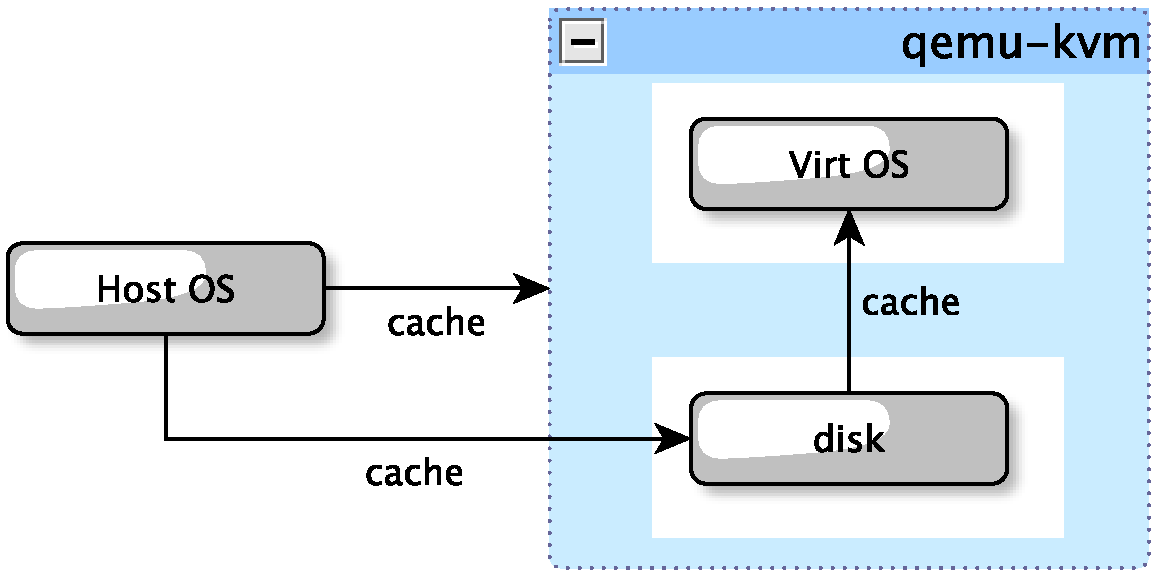
\includegraphics[width=\paperwidth/2]{data/cache.pdf}}
  \caption{Vyznačenie miest, kde môže nastať kešovanie}
  \label{graf-cache}
\end{center}
\end{figure}

Virtualizovaný systém musí obsahovať všetky potrebné balíčky, ktorých programy
sa používajú v testoch. Spúštanie testov bude prebiehať cez ssh spojenie a
preto je potrebné si zabezpečiť bezchybnú komunikáciu medzi hostiteľským a
virtualizovaným systémom - ideálne certifikát bez hesla pre root užívateľa a
statickú IP adresu, ktorá sa nezmení po reštarte systému.

\section{Použitie virtuálneho stroja}

\chapter{Záver}
Zaver

